\documentclass[a4paper]{article}
\usepackage{qtree}
\usepackage{forest}
\usepackage{multicol}
\setlength{\columnsep}{3cm}
\usepackage{parskip}
\usepackage{changepage}
\usepackage[T1]{fontenc}
\usepackage{amsmath}
\usepackage{listings}
\usepackage{amsthm}
\usepackage{amssymb}
\usepackage{float}
\usepackage[utf8]{inputenc}
\usepackage{graphicx}
\usepackage[italian]{babel}
\usepackage{thmtools}
\newtheorem*{theorem}{Teorema}
\newtheorem*{definition}{Definizione}
\newtheorem{example}{Example}
\newenvironment{dimostrazione}{\textit{Dimostrazione}:\begin{adjustwidth}{1cm}{}}{\end{adjustwidth}}

\begin{document}

\author{Lorenzo Dentis, lorenzo.dentis@edu.unito.it}
\title{Risposte AlgComp}
\maketitle

\section{Brute-force e certificazione}
\subsection{A.1}
Posto un array $V$ di $n$ elementi individuo due indici, $i$ e $j$.\\L'idea è di mantenere gli elementi $[0 ... j-1]$ fissi ed andare a generare tutte le permutazioni dei restanti elementi $[j ... n-1]$grazie all'indice $i$.

Ad ogni incremento dell'indice $i$ segue una sequenza di chiamate ricorsive che hanno lo scopo di effettuare uno swap fra l'elemto di indice $i$ e l'elemento di indice $j$ e poi incrementare $j$ scendendo nell'albero della ricorsione fino alla condizione $j=i$, quando $i$ viene di nuovo incrementato.Intuitivamente $j$ indica la profondità della ricorsione, $i$ indica l'ampiezza.
\begin{itemize}
	\item \textbf{Punto 1}:L'algoritmo è completo in quanto genera $n!$ permutazioni, ed è corretto in quanto sono tutte distinte.\\Le permutazioni generate sono esattamente $n!$ in quanto alla "radice" dell'albero avrò $n$ chiamate ricorsive (con $i = 0, i=1, ... i= n-2, i=n-1$ ).Invece al livello di profondità $j$ i primi $j$ elementi del vettore risulteranno fissi ed avrò solo $n-1-j$ chiamate ricorsive.\\Considerando che il valore di $j$ viene incrementato di una unità ad ogni "livello" di ricorsione fino all' $n-(n-1)$esimo livello ottengo questa semplice equazione: \begin{center}$calls = n * (n-1) * ...(j-1$volte$)... * 1$\end{center}Che non è altro che $n!$\\
		Le permutazioni sono tutte distinte perchè $i$ e $j$ non assumono mai due volte lo stesso valore, posto che ogni elemento del vettore sia distinto.Di conseguenza lo "swap" avverrà sempre tra due elementi differenti ad ogni chiamata ricorsiva, generando sottoalberi uno diverso dall'altro e di conseguenza sequenze differenti.
	\item \textbf{Punto 2}:Un algoritmo che generi \textit{tutti i sottoinsiemi di elementi} può essere realizzato organizzando lo spazio degli stati in sottoinsiemi.
		Al posto che intendere una permutazione come sequenza di elementi la si può vedere come una serie di \textit{scelte}, ovvero booleani.Essenzialmente si va a generare un vettore $B$ di booleani i cui elementi indicano se il corrispondente elemento di $V$ va considerato o meno.\\
		Se $B[i] == True$ allora $V[i]$ fa parte del sottoinsieme che si sta generando.\\
		In tal modo otteniamo il \textbf{PowerSet} di $V$, che è completo (cioè le permutazioni sono $2^n$) in quanto ogni cella del vettore $B$ può avere solamente valore binario e le celle sono $n$.
		E' invece corretto, di nuovo posto che gli elementi siano distinti, in quanto non vi è alcuno \textit{"swap"} e nessuna sequenza è ripetuta più volte. Ogni sequenza di \textit{True/False} varia dalla precedente di una scelta, garantendo sequenze distinte.
\end{itemize}
\begin{figure*}[!ht]
\centering
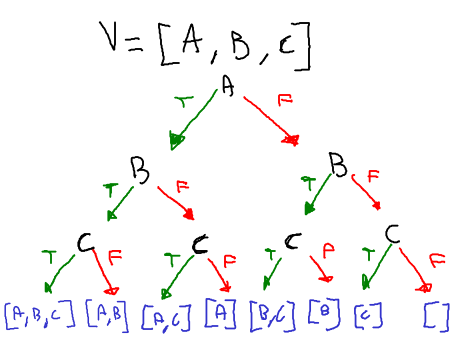
\includegraphics[scale = 0.5]{./img/A1_2.png}
\caption{PowerSet di [a,b,c]} \label{FIG:PowerSet}
\end{figure*}
\subsection{A.2}
Definizione formale di una permutazione (definizione ricorsiva):
\begin{figure*}[!ht]
\centering
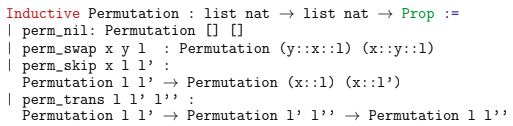
\includegraphics[width=0.7\textwidth]{./img/permutazione_ricorsiva.png}
\caption{Definizione ricorsiva di una permutazione} \label{FIG:recursive_permutation1}
\end{figure*}
\begin{itemize}
	\item perm\_nil: [ ] è permutazione di [ ] (lista vuota è permutazione di se stessa)
	\item perm\_swap: $\forall x,y \in Elements$ e $\forall l \in Lists$ $[y::x::l]$ e $[x::y::l]$ sono una permutazione dell'altra
	\item perm\_skip: dato $x \in Elements$, se $l \in Lists$ è permutazione di $l' \in Lists$ $\Rightarrow [x::l]$ è permutazione di $[x::l']$
	\item perm\_trans: date $l, l', l'' \in Lists$ se $l$ permutazione di $l'$ e $l'$ permutazione di $l'' \Rightarrow l$ è permutazione di $l''$ 
\end{itemize}
\begin{theorem}[Riflessività] $\forall l \in Lists$ Permutation $l$ $l$\end{theorem}
\textit{Dimostrazione}:
\begin{adjustwidth}{2cm}{}
	\textit{caso base}: $l$ = [ ], vale per definizione grazie a perm\_nil\\
	\textit{caso induttivo}: $l = [h::t]$ con $h \in Lists$ e $t \in ELements$.\\
	Grazie all'ipotesi induttiva si può affermare \textit{Permutation} $t$ $t$ e quindi per perm\_skip \textit{Permutation} $[h::t]$ $[h::t]$. Dato che $l = [h::t]$ abbiamo che \textit{Permutation} $l$ $l$.
\end{adjustwidth}
\begin{theorem}[Simmetria] $\forall l,l' \in Lists$, Permutation $l$ $l'$ $\Rightarrow $ Permutation $l$ $l'$\end{theorem}
\begin{dimostrazione}
	DA FAR
\end{dimostrazione}
\subsection{A.3}
Dimostrare che è algoritmo che genera permutazioni di una lista di elementi è completo significa dimostrare che genera $n!$ permutazioni, con $n$ pari al numero di elementi. Formalmente:
\begin{theorem}[Completezza] $\forall l \in Lists$, $len($\textit{permutation} $l) = len(l)!$\end{theorem}
\begin{dimostrazione}
	\textit{caso base}: $l$ = [ ]\\
	In questo caso $len(l)! = 0! = 1$.\\
	Allo stesso modo $len(permutation)$ [ ] $= len($[ [ ] ]$) = 1$.\\
	Quindi $len($\textit{permutation} $l) = len(l)!$
	
	\textit{Caso induttivo}: $l = h::t$, quindi l'enunciato da dimostrare è $len($\textit{permutation} $[h::t]) = len([h::t])!$\\
	$len(h::t) = 1 + len(t)$\\
	Quindi $len(distribute$ $a$ $[h::t]) = 2 + len(t)$ che per il Lemma distribute\_lenght diventa $len((a::t)::distribute$ $a$ $t) = 2 + len(t)$
	INSERIRE FOTO LEMMA DISTRIBUTE
\end{dimostrazione}
\subsection{A.4}
\begin{itemize}
	\item \textbf{Permutazioni}:Si può individuare una \emph{risposta} al problema \textbf{Valutazione} generando l'albero di tutte le possibili permutazioni:
		\begin{center}	\scalebox{0.8}{\Tree [  [ [ .1 [  [ .2 [.3 4 ] [.4 3 ] ] [ .3 [.2 4 ] [ .4 2 ] ] [ .4 [ .2 3 ] [ .3 2 ] ] ] ] [ .2 [ [ .1 [ .3 4 ] [ .4 3 ] ] [ .3 [ .1 4 ] [ .4 1 ] ] [ .4 [ .1 3 ] [ .3 1 ] ] ] ] [ .3 [ [ .1 [ .2 4 ] [ .4 2 ] ] [ .2 [ .1 4 ] [ .4 1 ] ] [ .4 [ .1 2 ] [ .2 1 ] ] ] ] [ .4 [ [ .1 [ .3 2 ] [ .2 3 ] ] [ .3 [ .1 2 ] [ .2 1 ] ] [ .2 [ .1 3 ] [ .3 1 ] ] ] ] ] ]}
		\end{center}
		In questo albero un ramo individua una permutazione dell'insieme di partenza, di conseguenza basta percorrerlo calcolando di volta in volta il voto massimo finchè questi non supera il valore fissato (in questa istanza 9).Si ottiene quindi una soluzione, data dalla sequenza di "voti" ottenuta partendo dalla radice e percorrendo il ramo corrispondente fino al padre del nodo che causa il superamento del voto massimo.
		Eseguendo questa operazione su tutti i rami dell'albero si ottengono tutte le \emph{soluzioni}, scegliendo le soluzioni con votazione migliore si ottengono una o più \emph{risposte}.
	\item \textbf{Sottoinsiemi}:Si può individuare una \emph{risposta} al problema \textbf{Valutazione} generando l'albero di tutte le possibili scelte:
		\begin{center}
			\begin{forest}
				for tree={ l sep=20pt, s sep=20pt}
			[1 [2, edge label = {node[midway,left,green] {T}} [3, edge label = {node[midway,left,green] {T}}[4, edge label = {node[midway,left,green] {T}}] [4, edge label = {node[midway,right,red] {F}}]] [3, edge label = {node[midway,right,red] {F}}[4, edge label = {node[midway,left,green] {T}}] [4, edge label = {node[midway,right,red] {F}}]]][2, edge label = {node[midway,right,red] {F}} [3, edge label = {node[midway,left,green] {T}}[4, edge label = {node[midway,left,green] {T}}] [4, edge label = {node[midway,right,red] {F}}]] [3, edge label = {node[midway,right,red] {F}}[4, edge label = {node[midway,left,green] {T}}] [4, edge label = {node[midway,right,red] {F}}]]]] 			\end{forest}
		\end{center}
		A seconda che si scelga un ramo o l'altro la domanda sarà inclusa nella possibile \emph{soluzione} quindi percorrendo un ramo fino alla foglia si giunge sempre ad una sequenza di voti.
		Non tutti i sottoinsiemi così generati sono però \emph{soluzioni}, in quanto alcuni superano il vincolo del voto massimo ammesso (in questo caso 9); considerando solo le \emph{soluzioni} e scegliendo quelle aventi la migliore votazioni si ottengono una o più \emph{risposte}
\end{itemize}
\section{Backtrack}
\section{Branch\&Bound}
\subsection{C.7}
Guarda la scacchiera come una matrice di 1 e 0
\subsection{C.14}
Nella creazione di un algoritmo \textit{Branch\&Bound} per \emph{KP} la prima cosa da fare è stabilire una \textbf{funzione costo}.Questo può essere fatto basandosi sulla gerarchia dei profitti degli algoritmi greedy vista in precedenza.In particolare il costo ad un \textit{E-node} $x[0..j)$ può essere scritto come:
$$\hat{c}(x[0..j)) = f(h(x[0..j))) + \hat{g}(x[0..j))$$
\begin{itemize}
	\item Nella prima parte dell'equazione abbiamo il \textit{costo noto}, che non è altro che la somma di tutti i profitti dei nodi "inseriti nello zaino" fin'ora ed i loro pesi. 
		\begin{equation}
                	f(h(x[0..j))\begin{cases}
			fh.w(x[0..j))= \sum_{0\leq k < j} x_{k}w_{k}\\
			fh.z(x[0..j))= \sum_{0\leq k < j} x_{k}p_{k}\notag
                \end{cases}
	        \end{equation}
	\item La seconda parte di equazione fornisce una stima per eccesso del profitto ottenibile (\textit{Upper bound}).
		\begin{equation}
			\hat{g}(x[0..j))\begin{cases}
				\hat{g}.w(x[0..j))= (\sum_{j\leq k < split} w_{k})+(c-[fh.w(x[0..j)) + \sum_{j\leq k < split} w_{k}]\\
				\hat{g}.z(x[0..j))= (\sum_{j\leq k < split} p_{k})+(c-[fh.w(x[0..j)) + \frac{\sum_{j\leq k < split} w_{k}]}{W_{split}}P_{split} \notag
                	\end{cases}
	        \end{equation}
	\item Una terza misura utile a scrivere un algoritmo \textit{Branch\&Bound} per il problema Knapspack è una stima per difetto (\textit{Lower Bound}), facilmente ottenibile tramite l'algoritmo greedy (o greedy split).
		\begin{align}
				z^g(x[0..j)) &= \sum_{0\leq k < j} x_{k}p_{k} + \sum_{j\leq k < split} p_{k} + \sum_{split < k < n} x_{k}p_{k} \notag \\
			&se \sum_{0\leq k < j} x_{k}w_{k} + \sum_{j\leq k < split} w_{k} + \sum_{split < k < n} x_{k}w_{k}\notag
		\end{align}
\end{itemize}
Una volta descritte le 3 misure si può impostare un algoritmo per la risoluzione \textit{Branch\&Bound} che rispetti la seguente invariante: In qualsiasi istante della visita $lower \; bound < z^* < upper \; bound$\\
L'idea di base è quindi quella di raffinare tramite le diverse iterazioni i due limiti fino ad ottenere la miglior \emph{soluzione} che sarà la \emph{risposta}.\\
\textit{Passo base}:
\begin{adjustwidth}{.8cm}{0cm}
		Non avendo visitato alcun nodo l' \textit{E-node} è la radice dello spazio degli stati.
		Il \textit{lower bound} è quindi l'algoritmo greedy scelto applicato al problema completo, allo stesso modo l' \textit{upper bound} è il risultato dell'algoritmo di soluzione di \emph{LKP} applicato al problema completo.
		In questo stadio la miglior soluzione (che identifichiamo come $x[0..r)$) è la soluzione trovata tramite l'algoritmo greedy.
\begin{figure*}[!ht]
\centering
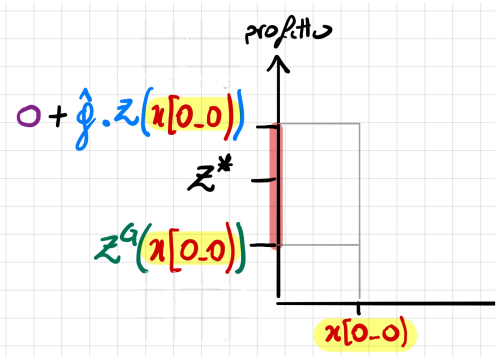
\includegraphics[width=0.7\textwidth]{./img/C14_profitto_z.png}
\caption{Bounds del profitto z} \label{FIG:C14_profitto_z}
\end{figure*}\\
\end{adjustwidth}
\textit{Passo induttivo}:
\begin{adjustwidth}{.8cm}{0cm}
	Al passo induttivo l'attuale \textit{E-node} sarà $x[0..j)$ e il nodo che fornisce la miglior soluzione $x[0..r)$ garantisce un profitto $z^*(x[0..r))$.
	Durante la visita dell' \textit{E-node} si possono presentare 4 situazioni (non esclusive):
	\begin{itemize}
		\item $f(h(x[0..j)) > C$\\
			Non ha senso "espandere" il nodo e proseguire nella visita del sotto-albero $T[0..j)$ in quanto sicuramente non otterremo una risposta avendo superato la capacità massima.Il nodo viene etichettato come \textbf{"completo"}, si sta effettuando \textit{pruning}.
		\item$f(h(x[0..j)) + \hat{g}.z(x[0..j)) < z^*(x[0..r))$\\
			Il profitto ottenibile espandendo il nodo è < dell'approssimazione per difetto trovata in uno dei passi precendenti.Anche inserendo tutti gli oggetti fino a capienza massima non si troverebbe una soluzione migliore di quella attuale (ricordo essere $z^*(x[0..r))$).Il nodo viene etichettato come \textbf{"completo"}, si sta effettuando \textit{pruning}.
\begin{figure*}[!ht]
\centering
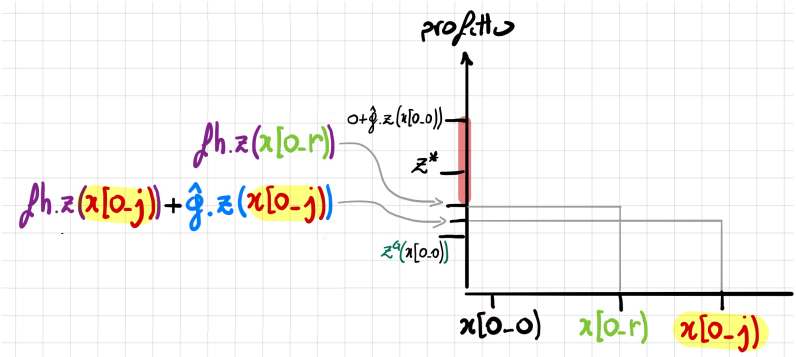
\includegraphics[width=0.7\textwidth]{./img/C14_item2.png}
\caption{nessun miglioramento rispetto alla soluzione del nodo $x[0..r)$} \label{FIG:C14_item2}
\end{figure*}\\
		\item $f(h(x[0..j)) < C \land f(h(x[0..j)) + \hat{g}.z(x[0..j)) > z^*(x[0..r))$\\
			Il sottoalbero $T[0..j)$ può ancora generare \textit{soluzioni}, fra queste potrebbe essere presente la \textit{risposta}.E quindi necessario \textbf{espandere} il nodo e continuare l'esplorazione del sottoalbero.
		\item $f(h(x[0..j)) < C \land f(h(x[0..j)) > z^*(x[0..r))$\\
			E' stata trovata una \textit{soluzione} che migliora il profitto $z^*(x[0..r))$, viene salvata ed i passi successivi faranno riferimento al profitto generato da $x[0..j)$.
	\end{itemize}
	\begin{figure*}[!ht]
\centering
\textbf{$((2,4,6,9),(10,10,12,18),15) \in KP$}
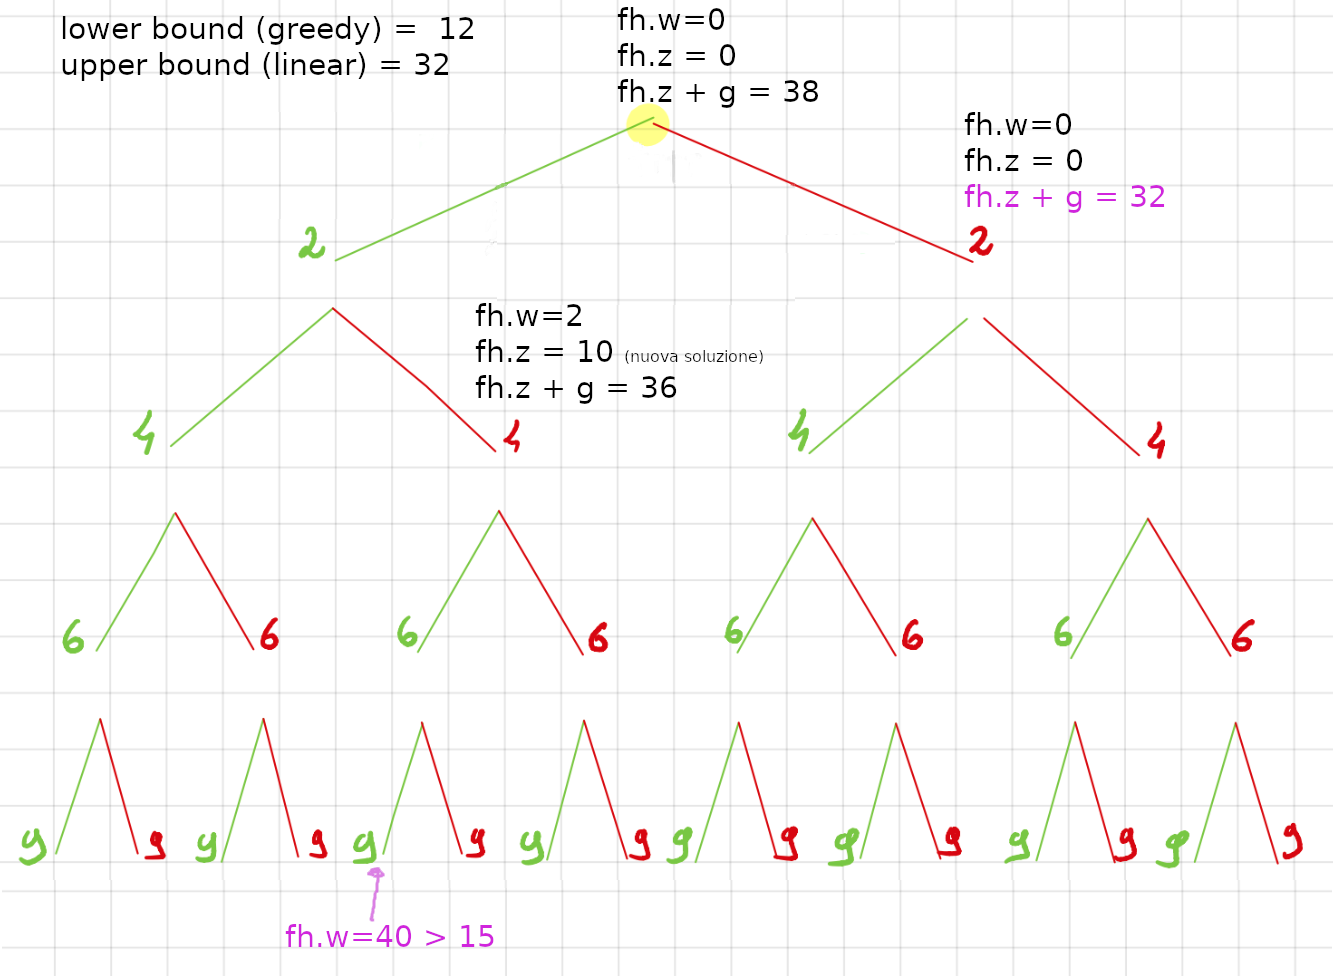
\includegraphics[width=1\textwidth]{./img/C14_BB_manuale.png}
\caption{Esempio di Branch\&Bound} \label{FIG:C14_BB_manuale}
\end{figure*}
	La cosa non specificata dall'algoritmo è il criterio di scelta del prossimo \textit{E-node} tra i vari \textit{live-nodes} disponibili.Utilizzando un criterio FIFO si ottengono buoni risultati, ma usando una tecnica \emph{least-cost} si è scoperto sperimentalmente che le prestazioni sono migliori.
	Intuitivamente ci sono due motivi per questo: in primis se $z^{LP} = Z^*$ è possibile che venga trovata una soluzione che sappiamo con certezza essere anche \textit{risposta}, si può quindi fare pruning dei restanti rami.
	In secondo luogo è possibile che giungendo "prima" alle \textit{soluzioni} migliori il valore di $z^*(x[0..r))$ cresca rapidamente causando il "rifiuto" di nodi che con una politica FIFO sarebbero stati espansi.(I nodi vengono rifiutati per la situazione 2)
%si può parlare brevemente anche di come scegliere i nodi, FIFO vs LC
\end{adjustwidth}
\section{Problemi computazionali}
\subsection{D.2}
Dimostrare che i problemi \emph{KP} e \emph{Bounded-KP} sono equivalenti.\\Cioè $KP \Leftrightarrow BKP$.\\
\begin{dimostrazione}
	$KP \Rightarrow BKP$: ogni problema \emph{KP} è un problema \emph{BKP}.\\
	La dimostrazione è immediata in quanto un generico problema\\$((P_1, ... ,P_n),(W_1, ... ,W_n),C)\in KP$ può essere riscritto come\\ $((P_1, ... ,P_n),(W_1, ... ,W_n),(1, ... ,1),C) \in BKP$.

	$KP \Leftarrow BKP$: ogni problema \emph{BKP} è un problema \emph{KP}.\\
	per prima cosa introduciamo $B_i + 1$ nuove variabili, $\forall i \in B_1 ... B_n$.\\
	Avremo quindi
	\begin{align}
		x_{0}', ... ,&x_{b_i}' \in \{0,1\}  \notag \\
   		&\;\;\vdots \notag \\
		x_{0}^n, ... ,&x_{b_i}^n \in \{0,1\}  \notag 
	\end{align}
	Queste variabili indicano "quanti" oggetti di tipo $x^i$ sto prendendo, quindi 
	\begin{equation}
		x_{j}^i=\begin{cases}
      		0\; se\; x_i = 0\\
      		1\; se\; x_i = j \notag
    		\end{cases}
	\end{equation}
	Il problema è diventato un esempio di \emph{BKP} di questo tipo:
	\begin{center}
		\scalebox{0.89}{$((p_1, 2p_1 ,...,b_1p_1, ... ,p_n, 2p_n, ..., b_np_n),(w_1, 2w_1 ,...,b_1p_1, ... ,w_n, 2w_n, ..., b_nw_n),C))$}\\
		$maximize \; \sum_{i=1}^{n} \sum_{j=0}^{b_i} p_j*j*x^i_j$\\
		$subject \; to \; \sum_{i=1}^{n} \sum_{j=0}^{b_i} w_j*j*x^i_j$\\
		con la condizione aggiuntiva $ \forall i \sum_{j=0}^{b_i} x_j^i = 1$
	\end{center}
	In modo che  si possano prendere solo $j$ oggetti fi tipo $x^i$
	%non posso prendere 5 x', e poi 3 x', sarebbe come prendere 8 x'
	DA FINIRE CON OSSERVAZIONE DEL PROF RIGUARDO AL FATTO DI DOVER DIMOSTRARE LA RISOLVIBILITà
\end{dimostrazione}
\end{document}
